\chapter{テスト粒子で円盤銀河を作る}
\label{chap:ch4}

第3章では、固定したPlummerポテンシャル中で1個の星を動かしました。この章では、同じ重力場の中に多数の星を配置し、回転する円盤を作ります。新しく学ぶ数値計算法は線形補間です。前章の台形則と乱数を組み合わせ、指定した分布に従う粒子の位置を生成します。時間発展には、引き続きleapfrog法のkick--drift--kick（KDK）形式を使います。

ここで作るのは、自己重力で支え合う円盤ではありません。重力はPlummer球が作り、星を表すテスト粒子はその重力を受けるだけです。粒子を多数に増やすことと、粒子同士の重力を計算することを区別します。まず一つの銀河の中で円盤が保たれることを確かめ、第5章の相互作用へ進む準備をします。

\begin{goalbox}[この章で学ぶこと]
\begin{itemize}
\item 円盤の面密度と、粒子の半径の確率密度の違いを説明できます。
\item 台形則で累積分布関数を作り、線形補間で逆変換できます。
\item 乱数から位置を生成し、同じPlummerモデルの円運動速度を与えられます。
\item 1粒子の加速度をNumPyで多数粒子へ拡張し、KDKで時間発展させられます。
\item 分布表の誤差、有限粒子数のばらつき、軌道積分の誤差を分けて確認できます。
\end{itemize}
\end{goalbox}

\section{重力を作る球と表示する円盤を区別する}
\label{sec:ch4-model}
\subsection{本章のモデルを定義する}
原点に質量$M$、スケール長$a$のPlummer球を固定します。ポテンシャルは前章と同じ
\begin{equation}
\Phi(r)=-\frac{GM}{\sqrt{r^2+a^2}}
\label{eq:ch4-potential}
\end{equation}
です。\cite{bt2008}球の質量は時間によらず一定で、粒子の配置を変えても変わりません。質量をもたないテスト粒子を$x$--$y$平面に置き、初期速度もその平面内で与えます。外部からの力、ガス、星形成、動力学的摩擦は含めません。

粒子$i$の位置と速度は$\rvec_i=(x_i,y_i)$、$\vvec_i=(v_{x,i},v_{y,i})$です。円盤の中心からの半径を$R=\sqrt{x^2+y^2}$と書きます。重力を作る球の半径$r=\sqrt{x^2+y^2+z^2}$とは定義が異なりますが、本章では$z=0$なので$r=R$です。$R$はここでは円盤の半径であり、後の銀河中心の位置ベクトル$\Rvec_k$ではありません。

\subsection{円盤の粒子に質量を割り当てない}
画面上に円盤が現れても、その粒子分布から重力場を計算しているわけではありません。Plummer球の質量$M$を$N$等分して粒子へ配る操作も行いません。$M$は背景ポテンシャルのパラメータで、$N$は円盤を描くために追跡する粒子数です。

本章では円盤の形を\textbf{粒子数面密度}$\Sigma_N$で定義します。これは面積当たりの粒子数です。各粒子に同じ表示上の重みを与えれば恒星分布の形を表せますが、その重みを加速度計算へ入れることはしません。このため、円盤の分布とPlummer球の密度は独立に選べます。自分自身の重力まで含めた平衡銀河を構成する問題とは、区別してください。

\begin{failbox}{多数の粒子があっても、相互重力はまだありません}
各粒子は同じ解析的ポテンシャルから独立に力を受けます。粒子数を2倍にしても、すでに置いた1粒子への力は変わりません。本章は多数のテスト粒子の計算であり、自己重力円盤のN体計算ではありません。
\end{failbox}

\section{指数円盤を半径の確率分布へ直す}
\label{sec:ch4-probability}
\subsection{初期の配置範囲を決める}
中心ほど粒子が多い円盤を作るため、初期の粒子数面密度を
\begin{equation}
\Sigma_N(R)=\Sigma_{N,0}\exp(-R/R_d),\qquad 0\le R\le R_{\max}
\label{eq:ch4-surface-density}
\end{equation}
とします。$R_d$は指数分布のスケール長、$R_{\max}$は初期粒子を配置する外縁です。この形は構成案で選んだ教材用モデルです。本章では$R_d=a=3\unit{kpc}$としますが、二つは同じ物理量ではなく、等しくする必要もありません。

第3章の$r_{\rm tab}$は、無限遠まで続くPlummer球の質量表を作る範囲でした。一方、今回は初期粒子分布を$R_{\max}$で切断すると\emph{定義}しています。ただし、Plummer球の密度や重力をそこで切断しません。また、時間積分中に$R_{\max}$を越えた粒子を取り除いたり、跳ね返したりもしません。初期の配置範囲と、運動の境界条件は別です。

\subsection{円環の面積を含める}
半径$R$から$R+dR$までの薄い円環の面積は$2\pi R\,dR$です。その中の期待粒子数は
\begin{equation}
dN=2\pi R\Sigma_N(R)\,dR
\label{eq:ch4-annulus}
\end{equation}
となります。全粒子数で割れば、半径の確率密度$p_R(R)$が得られます。
\begin{equation}
p_R(R)=\frac{2\pi R\Sigma_N(R)}{N}
       =\frac{R\exp(-R/R_d)}{\displaystyle\int_0^{R_{\max}}R'\exp(-R'/R_d)\,dR'}.
\label{eq:ch4-radial-pdf}
\end{equation}
$p_R$の単位は長さの逆数です。$p_R(R)\,dR$は無次元の確率であり、面密度とは異なります。第3章の球殻には$4\pi r^2$を使いましたが、ここで粒子を配置するのは円盤なので$2\pi R$です。

$\Sigma_N$は中心で最大ですが、$p_R(0)=0$です。中心に近い円環ほど面積が小さいからです。$R_{\max}>R_d$なら、$R\exp(-R/R_d)$を微分すると、半径の確率密度は$R=R_d$で最大になります。中心に面密度のピークがあることと、半径のヒストグラムのピークが中心にあることは同じではありません。


% BEGIN TikZ addition: ch04_annulus
図\ref{fig:concept-ch4-annulus}では、円環の面積と二つの分布の違いを対応させています。第3章の球殻（図\ref{fig:concept-ch3-shell}）と比べ、今回は体積ではなく面積を掛けることを確認してください。
\begin{figure}[!htbp]
\centering
% Geometry and two dimensionless density functions, not a simulated snapshot.
\begin{tikzpicture}[textbook diagram]
  \node[anchor=west,font=\sffamily\bfseries] at (0,4.9) {Area matters when sampling a radius};
  \coordinate (O) at (2.4,2.45);
  \draw[guide] (O) circle (2.0);
  \path[fill=figblue!12,even odd rule] (O) circle (1.38) (O) circle (1.16);
  \draw[figblue] (O) circle (1.16);
  \draw[figblue] (O) circle (1.38);
  \fill (O) circle (1.3pt);
  \draw[vector] (O) -- ($(O)+(30:1.16)$) node[midway,above left] {$R$};
  \draw[guide] ($(O)+(135:1.16)$) -- (0.55,3.72);
  \draw[guide] ($(O)+(135:1.38)$) -- (0.35,3.92);
  \node[anchor=east] at (0.48,3.93) {$dR$};
  \node[anchor=west] at (3.4,4.10) {$R_{\max}$};
  \node at (2.4,-0.15) {$dA=2\pi R\,dR$};
  \node[small label,text=figgray] at (2.4,-0.67) {Ring thickness exaggerated};
  \begin{scope}[shift={(6.0,0.65)},x=1cm,y=3.05cm]
    \draw[vector] (0,0) -- (5.15,0) node[right] {$R/R_d$};
    \draw[vector] (0,0) -- (0,1.15);
    \node[rotate=90,small label] at (-0.88,0.56) {Dimensionless density};
    \foreach \x in {0,1,2,3,4,5} {\draw (\x,0) -- (\x,-0.027); \node[below,small label] at (\x,-0.027) {\x};}
    \foreach \yy in {0.5,1.0} {\draw (0,\yy) -- (-0.065,\yy); \node[left,small label] at (-0.065,\yy) {\yy};}
    \draw[figblue,line width=0.95pt,domain=0:5,samples=81] plot (\x,{exp(-\x)});
    \draw[figred,line width=0.95pt,dashed,domain=0:5,samples=81] plot (\x,{\x*exp(-\x)/(1-6*exp(-5))});
    \fill[figblue] (0,1) circle [radius=1.6pt];
    \draw[figred,fill=white] (1,{exp(-1)/(1-6*exp(-5))}) circle [radius=2pt];
  \end{scope}
  \draw[figblue,line width=0.95pt] (6.10,-0.35) -- (6.75,-0.35);
  \node[anchor=west] at (6.85,-0.35) {$\Sigma_N/\Sigma_{N,0}=e^{-R/R_d}$};
  \draw[figred,line width=0.95pt,dashed] (6.10,-1.00) -- (6.75,-1.00);
  \node[anchor=west] at (6.85,-1.00) {$R_d\,p_R(R)$};
  \node[small label,anchor=west,text=figgray] at (6.85,-1.50) {$R_{\max}=5R_d$; normalized on this range};
  \node[draw=black!30,fill=white,align=center,text width=106mm,inner sep=5pt] at (5.75,-2.45) {$dN=\Sigma_N(R)\,dA=2\pi R\,\Sigma_N(R)\,dR$};
\end{tikzpicture}

\caption{円環の面積と半径の確率密度の関係。面密度に$2\pi R$を掛けて半径の分布へ直します。右側は$R_{\max}=5R_d$で規格化した解析的な入力分布で、標本化した粒子の結果ではありません。面密度は中心で最大でも、半径の確率密度は中心で0です。}
\label{fig:concept-ch4-annulus}
\end{figure}
\FloatBarrier
% END TikZ addition: ch04_annulus

\begin{failbox}{半径を指数乱数にすればよい、とは限りません}
$p_R\propto\exp(-R/R_d)$としてしまうと、円環の面積に由来する$R$を落としてしまいます。また、$R$を一様乱数で選んでも、面積当たり一様な円盤にはなりません。何に対する密度を指定しているかを、最初に確認します。
\end{failbox}

\section{台形則で累積分布関数を作る}
\label{sec:ch4-cdf}
\subsection{半径以内に入る確率を求める}
半径$R$以内に入る確率を、累積分布関数（cumulative distribution function; CDF）と呼びます。ここでは
\begin{equation}
F(R)=\int_0^R p_R(R')\,dR'
=\frac{\displaystyle\int_0^R R'\exp(-R'/R_d)\,dR'}
       {\displaystyle\int_0^{R_{\max}}R'\exp(-R'/R_d)\,dR'}
\label{eq:ch4-cdf-definition}
\end{equation}
です。$F(0)=0$、$F(R_{\max})=1$で、その間で単調に増えます。累積分布とその逆関数から目的の分布に従う乱数を作る考え方は、文献\cite{irifuji1985}の第23章で扱われています。

解析的な比較値も用意できます。$x=R/R_d$、$x_{\max}=R_{\max}/R_d$として
\begin{equation}
C(x)\equiv 1-(1+x)e^{-x}
\label{eq:ch4-C}
\end{equation}
と置きます。$R'\exp(-R'/R_d)$を積分すると$R_d^2 C(R/R_d)$になるので、
\begin{equation}
F(R)=\frac{C(R/R_d)}{C(x_{\max})},\qquad
p_R(R)=\frac{R\exp(-R/R_d)}{R_d^2 C(x_{\max})}
\label{eq:ch4-cdf-exact}
\end{equation}
です。初期分布の規格化定数は$\Sigma_{N,0}=N/[2\pi R_d^2C(x_{\max})]$です。この式は本章の面密度を積分して得た比較用の式であり、数値CDFを作る処理には使いません。

$x_{\max}=5$では$C(x_{\max})=\chfourvalCq$です。無限に延ばした同じ指数分布のうち、約4.04\%が$5R_d$より外側にあります。本章ではそこを初期配置の対象から外し、内側の条件付き分布を確率1へ規格化します。Plummer球の$5a$以内の質量割合とは別の数です。

\subsection{前章の累積積分を再利用する}
分点を$R_j$、被積分関数を$g_j=R_j\exp(-R_j/R_d)$として、台形の面積を順に足します。
\begin{align}
I_0&=0, & I_{j+1}&=I_j+\frac{g_j+g_{j+1}}{2}(R_{j+1}-R_j),\label{eq:ch4-cumulative-trapezoid}\\
\widehat F_j&=\frac{I_j}{I_{N_R}}.\label{eq:ch4-numeric-cdf}
\end{align}
$N_R$は区間数で、分点数は$N_R+1$です。ハットは数値近似を表します。$I_j$の単位は長さの2乗ですが、最後の値で割った$\widehat F_j$は無次元です。

第3章では、有限範囲の累積質量を無条件に全質量$M$へそろえませんでした。ここで最後の値で割ってよいのは、式\eqref{eq:ch4-cdf-definition}そのものが\emph{有限範囲で規格化した確率}だからです。表を都合よく補正する操作ではありません。

\inputcode{chap04/trapezoid}

\subsection{標準条件でCDF表を実装する}
内部単位はkpc、Gyr、$\Msun$です。速度は内部ではkpc\,Gyr$^{-1}$を使い、表示するときだけkm\,s$^{-1}$へ換算します。質量・Plummerスケール長は第3章と共通です。その他の条件は、この章の孤立円盤を確認するために設定しました。
\inputcode{chap04/parameters}

\begin{table}[htbp]
\centering\small
\caption{第4章の標準条件。$N_R$、$N$、$N_{\rm step}$はそれぞれ別の個数です。$R_{\max}$はPlummer球の外縁ではありません。}
\label{tab:ch4-parameters}
\begin{tabular}{ll}\toprule
量 & 設定 \\\midrule
Plummer球 & $M=10^{11}\Msun$, $a=3\unit{kpc}$ \\
粒子の初期分布 & $R_d=3\unit{kpc}$, $R_{\max}=15\unit{kpc}=5R_d$ \\
粒子数・乱数seed & $N=1000$, seed $=42$ \\
CDFの区間数・分点数 & $N_R=4096$, $4097$分点 \\
回転方向 & $s_{\rm rot}=+1$（反時計回り） \\
終時刻・ステップ数 & $t_{\rm end}=0.60\unit{Gyr}$, $N_{\rm step}=3000$ \\
時間刻み・保存間隔 & $\Delta t=0.2\unit{Myr}$、10ステップごと \\\bottomrule
\end{tabular}
\end{table}

\inputcode{chap04/build-cdf}

\texttt{check\_positive}と\texttt{check\_integer}は、正で有限な値、正の整数であることを確認する補助関数です。完全なコードはNotebookに含めます。\texttt{cdf}を後で逆変換するため、隣接する値がすべて増えていることも確認します。標準条件では、$R=0$の被積分関数が0でも最初の台形の面積は正なので、CDFの最初の区間も増えます。

\begin{figure}[htbp]
\centering\includegraphics[width=0.73\linewidth]{\figpath{ch04_cdf}}
\caption{初期円盤のCDF。灰色破線は式\eqref{eq:ch4-cdf-exact}、青実線は台形則による数値表です。有限の初期配置範囲$[0,5R_d]$で規格化しています。}
\label{fig:ch4-cdf}
\end{figure}
分点上で解析式と比較した最大差は$\chfourvalNodeError$でした。図\ref{fig:ch4-cdf}ではほぼ重なりますが、この近似誤差が0という意味ではありません。

\section{線形補間で分点間の値を求める}
\label{sec:ch4-interpolation}
\subsection{2点間の関数を直線で近似する}
CDF表は、決めた分点の値しか持ちません。分点の間の値を求めるため、二つの点を結ぶ直線で近似します。この操作が線形補間です。前章の台形則では同じ直線の下の面積を求めましたが、ここでは直線上の値そのものを使います。

一般の表$(x_j,y_j)$について、$x_j\le x\le x_{j+1}$の位置を
\begin{equation}
\lambda=\frac{x-x_j}{x_{j+1}-x_j}
\label{eq:ch4-fraction}
\end{equation}
で表します。左端なら$\lambda=0$、右端なら$\lambda=1$です。二つの値をその割合で混ぜると、
\begin{equation}
y_{\rm lin}(x)=(1-\lambda)y_j+\lambda y_{j+1}
\label{eq:ch4-linear-interpolation}
\end{equation}
となります。分点では表の値に一致し、その間では両端の値の間を取ります。傾きを用いた$y_j+(y_{j+1}-y_j)(x-x_j)/(x_{j+1}-x_j)$とも同じ式です。補間と補間誤差の一般的な考え方は文献\cite{sugiura2009}の\S2.3を参照してください。

\subsection{一つの点を実装して確かめる}
まず区間を順に探す、短い実装を作ります。区間が見つかったら、式\eqref{eq:ch4-fraction}と式\eqref{eq:ch4-linear-interpolation}を計算するだけです。入力する分点は狭義単調増加とします。
\inputcode{chap04/linear-interpolation}
この関数は表の外では停止します。補間は表の内側での近似であり、外側へ直線を延ばす外挿とは区別します。\texttt{check\_grid}は第3章と同じく、分点・値の配列の形と有限性、分点の増加を確かめます。

多数の点を補間するときには、\texttt{np.interp(x, xp, fp)}を使います。\texttt{xp}が入力側の分点、\texttt{fp}がその値です。自作関数で原理を確認したうえで、同じ区分的な線形補間を行うライブラリ関数に置き換えます。\cite{numpy}全粒子についてPythonで表を繰り返し走査する必要はありません。

\begin{failbox}{増加していない表をそのまま渡さない}
入力側の分点に重複があると、式\eqref{eq:ch4-fraction}の分母が0になります。表を作る段階で、分点が有限で狭義単調増加かを確認します。また、\texttt{np.interp}は既定では表の外で端の値を返します。本章の自作関数とはこの扱いが違うので、呼び出し前に補間点が表の範囲内にあることを確認します。
\end{failbox}

\subsection{線形補間の精度と表の誤差を区別する}
真の関数$f$が滑らかで、両端の値が正しく与えられている場合、線形補間の誤差は区間内のある点$\xi$を使って
\begin{equation}
f(x)-f_{\rm lin}(x)=\frac{f''(\xi)}{2}(x-x_j)(x-x_{j+1})
\label{eq:ch4-interpolation-error}
\end{equation}
と書けます。区間幅を$h$とし、$|f''|$が上から抑えられるなら、誤差の大きさは$\max|f''|\,h^2/8$以下です。これが、滑らかな関数を細かい表で線形補間したとき、通常は幅の2乗で誤差が減る理由です。式は多項式補間の誤差公式の2分点の場合です。\cite{sugiura2009}

ただし、これから使うCDF表の値には台形則の誤差もあります。補間してもその誤差は消えません。さらに、CDFの逆関数は中心近くで傾きが大きくなるため、半径の誤差が全域で単純な同じ比例関係に従うとは限りません。本章では解析CDFに戻した確率のずれを、まず確認します。

\begin{notebox}{ほかの補間法}
多項式補間や三次スプラインは、より多くの分点を使って関数を近似します。高次の方法が有利な場合もありますが、点の間で振動したり、単調性を失ったりしないか確認が必要です。PCHIPは単調性を保つ区分的三次補間の代表例です。\cite{scipy_pchip}本章では、増加する表を扱いやすく実装も短い線形補間に集中します。詳細な理論と代替法の実装は数値計算の教科書に譲ります。
\end{notebox}

\section{一様乱数を円盤の半径へ変換する}
\label{sec:ch4-sampling}
\subsection{CDFの逆向きに表を読む}
$0\le u<1$の一様乱数を一つ選び、$F(R)=u$となる半径を求めます。CDFは「半径から確率」を返しますが、ここでは「確率から半径」を求めます。この方法を逆変換サンプリングと呼びます。\cite{irifuji1985}

なぜこれで正しい分布になるのでしょうか。単調増加する$F$では、生成半径が$R_*$以下になることと、一様乱数が$F(R_*)$以下になることが同値です。一様乱数がその範囲へ入る確率は$F(R_*)$です。このため、生成半径の累積分布は目標の$F$になります。実装では、これを数値表の逆補間で近似します。

$\widehat F_j\le u\le\widehat F_{j+1}$なら、入力側を$\widehat F$、出力側を$R$として
\begin{equation}
\widehat R(u)=R_j+
\frac{u-\widehat F_j}{\widehat F_{j+1}-\widehat F_j}(R_{j+1}-R_j)
\label{eq:ch4-inverse-interpolation}
\end{equation}
です。$\widehat F_j$が増えているので、$\widehat R$は必ず二つの分点の間に入ります。
\inputcode{chap04/inverse-example}
標準表で$u=0.5$を逆変換すると、半径は$\chfourvalHalfInterp\unit{kpc}$でした。自作関数と\texttt{np.interp}の値が一致することを確認します。これは初期円盤の\emph{粒子数}の半分を含む半径で、Plummer球の半質量半径ではありません。

図\ref{fig:ch4-interpolation}の矢印を、縦軸の確率から横軸の半径へたどってください。

\begin{figure}[htbp]
\centering% The original numerical line and analytic CDF are embedded unchanged.
\begin{tikzpicture}[textbook diagram]
  \node[inner sep=0,anchor=south west] (plot) at (0,0) {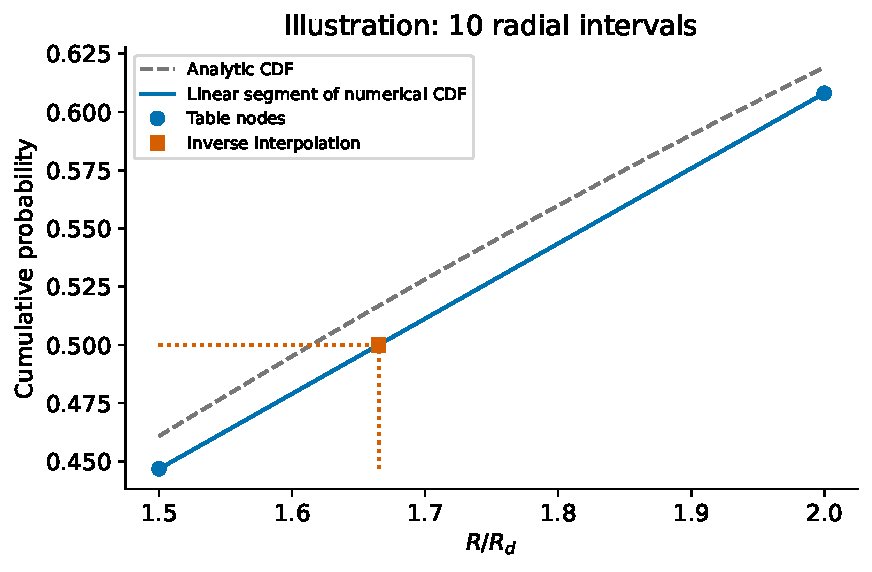
\includegraphics[width=118mm]{figures/ch04_interpolation.pdf}};
  \begin{scope}[x={(plot.south east)},y={(plot.north west)}]
    \draw[vector,figred] (.147,.396700) -- (.422,.396700);
    \draw[vector,figred] (.433970,.380) -- (.433970,.146);
    \node[small label,fill=white,inner sep=1pt,above] at (.245,.402) {$u=0.5$};
    \node[small label,fill=white,inner sep=1pt,anchor=west] at (.453,.196) {$\widehat R(u)/R_d$};
    \node[small label,fill=white,inner sep=1.5pt,anchor=west] (lo) at (.24,.198) {$(R_j,\widehat F_j)$};
    \draw[guide] (lo.west) -- (.182204,.180028);
    \node[small label,fill=white,inner sep=1.5pt,anchor=east] (hi) at (.905,.545) {$(R_{j+1},\widehat F_{j+1})$};
    \draw[guide] (hi.east) -- (.944684,.836223);
  \end{scope}
\end{tikzpicture}

\caption{数値CDFの一つの線分を逆向きに読む例。説明用に10区間だけで作った粗い表を使っています。丸が分点、四角が$u=0.5$の逆補間です。灰色破線の解析CDFとの差も示しています。標準の4096区間の結果とは区別してください。朱色の矢印は$u$から線分へ、そこから$\widehat R(u)$へ読む順序です。表の組$(R_j,\widehat F_j)$を示し、横軸では$R$を$R_d$で規格化しています。}
\label{fig:ch4-interpolation}
\end{figure}

\subsection{乱数を使う前に、逆変換を検証する}
同じ数値表で$u\to\widehat R\to\widehat F$と戻せば、線形補間の範囲ではもとの$u$にほぼ戻ります。しかし、それだけでは数値表が正しいかは分かりません。比較には、独立な解析CDFである式\eqref{eq:ch4-cdf-exact}を使います。

まず分点上の誤差$e_{F,\rm node}$を、次に固定した確率の集合$\mathcal U$上の逆変換の誤差$e_u$を
\begin{align}
e_{F,\rm node}&=\max_j|\widehat F_j-F(R_j)|,\label{eq:ch4-node-error}\\
e_u&=\max_{u\in\mathcal U}|F(\widehat R(u))-u|\label{eq:ch4-inverse-error}
\end{align}
で定義します。本章の$\mathcal U$は0から1までの20001個の等間隔の点です。まだ乱数は使いません。$e_u$は選んだ試験点上の最大値であって、連続な全確率範囲の最大誤差を厳密に保証する値ではありません。
\inputcode{chap04/cdf-convergence}

\begin{table}[htbp]
\centering\small
\caption{CDFの分割数試験。範囲$[0,5R_d]$と試験確率は固定しています。$p_u$は隣接する行の$e_u$の比から求めた推定次数です。}
\label{tab:ch4-cdf-convergence}
\begin{tabular}{rrrrr}\toprule
$N_R$ & $\Delta R\ [\mathrm{kpc}]$ & $e_{F,\rm node}$ & $e_u$ & $p_u$ \\
\midrule
32 & 0.468750 & $1.52\times 10^{-3}$ & $2.45\times 10^{-3}$ & --- \\
64 & 0.234375 & $3.80\times 10^{-4}$ & $6.98\times 10^{-4}$ & 1.8117 \\
128 & 0.117188 & $9.51\times 10^{-5}$ & $1.85\times 10^{-4}$ & 1.9121 \\
256 & 0.058594 & $2.38\times 10^{-5}$ & $4.80\times 10^{-5}$ & 1.9486 \\
512 & 0.029297 & $5.94\times 10^{-6}$ & $1.12\times 10^{-5}$ & 2.0986 \\
\bottomrule\end{tabular}

\end{table}
\begin{figure}[htbp]
\centering\includegraphics[width=0.72\linewidth]{\figpath{ch04_cdf_convergence}}
\caption{数値CDFと逆補間による確率のずれ。点線は最も細かい分割の値を通る傾き2の参照線で、当てはめではありません。試験確率が有限個なので、最大誤差の位置の拾い方も推定次数に影響します。}
\label{fig:ch4-cdf-convergence}
\end{figure}

表\ref{tab:ch4-cdf-convergence}では、分割を細かくすると誤差が減っています。標準の4096区間での$e_u$は$\chfourvalInverseError$でした。この数値誤差と、次に見る有限粒子数のばらつきを分けて考えます。表を細かくするだけで、乱数で配置した点が完全になめらかな分布になるわけではありません。

\subsection{半径と方位角に乱数を与える}
半径のための$u_i$とは別に、一様乱数$w_i$を使って$\phi_i=2\pi w_i$とします。ここで$\phi$は方位角です。二つを独立に選ぶことで、半径によらず方位角を一様にできます。位置は
\begin{equation}
x_i=R_i\cos\phi_i,\qquad y_i=R_i\sin\phi_i
\label{eq:ch4-polar-position}
\end{equation}
です。同じ乱数一つを半径と角度に流用すると両者が関連し、意図した軸対称の分布を作れません。

Notebookでは\texttt{rng = np.random.default\_rng(seed)}で乱数生成器を用意します。\texttt{rng.random((N, 2))}の各行に、半径と角度に使う二つの一様乱数を入れます。seedは実験を再現するための設定です。同じ実装・乱数生成環境・呼び出し順序なら同じ初期値を再現できますが、seedだけで異なる実装や将来のライブラリ環境まで同一の乱数列になると保証はしません。\cite{numpy}配布物には初期配列と使用したNumPyの版も記録します。

\begin{notebox}{ほかの標本化法}
棄却法は、候補の乱数を生成し、目標分布に応じて採用するかを選ぶ方法です。逆関数を求めにくい場合にも使えます。本書では、既習の台形則と今回の補間を一つの計算へ結び付けるため、CDFの逆変換を使います。乱数による積分を含むMonte Carlo法の一般論は、文献\cite{irifuji1985}に譲ります。
\end{notebox}

\section{円運動速度を与えて円盤を作る}
\label{sec:ch4-initial}
\subsection{同じ重力場から初期速度を求める}
粒子を置くだけでは、円盤を回転させたことにはなりません。各半径でPlummer球の円運動速度を与えます。第3章の式を再利用すると、
\begin{equation}
v_c^2(R)=\frac{GMR^2}{(R^2+a^2)^{3/2}}
\label{eq:ch4-circular-speed}
\end{equation}
です。粒子の分布のスケール長$R_d$を、この分母の$a$へ取り違えないようにします。位置の確率を決める式と、重力を決める式は別です。

反時計回りの接線方向の単位ベクトルは$(-\sin\phi,\cos\phi)$です。回転方向を$s_{\rm rot}=+1$または$-1$として、
\begin{equation}
v_{x,i}=-s_{\rm rot} v_c(R_i)\sin\phi_i,\qquad
v_{y,i}=s_{\rm rot} v_c(R_i)\cos\phi_i
\label{eq:ch4-circular-velocity}
\end{equation}
と置きます。例えば正の$x$軸上の粒子は、$s_{\rm rot}=+1$なら正の$y$方向へ動き始めます。すべての粒子に同じ\emph{速度の大きさ}を与えるのではなく、それぞれの$R_i$に対応する$v_c$を使います。

本章の孤立円盤には、もう一つの銀河の軌道はありません。そのため、ここでは反時計回り・時計回りと呼びます。遭遇軌道の向きとの関係で定義するprograde・retrogradeは、第5・6章で扱います。

\inputcode{chap04/plummer-speed}
\subsection{位置と速度を一つの初期配列へまとめる}
半径の標本化、方位角、接線速度を一つの関数にまとめます。位置と速度はそれぞれ形$(N,2)$です。最後に横に並べ、各行に$[x,y,v_x,v_y]$を持つ形$(N,4)$の状態配列を返します。
\inputcode{chap04/make-disk}

標準例では、\texttt{rng = np.random.default\_rng(seed)}を用意して\texttt{make\_disk}に渡します。乱数生成器を関数の中で毎回同じseedへ戻しません。比較実験でまったく同じ初期標本を使う場合だけ、同じseedの生成器を改めて作ります。初期粒子の半径は、今回の標本では約$\chfourvalMinRadius$から$\chfourvalMaxRadius\unit{kpc}$でした。上限15 kpc以内であることを確認します。

\begin{figure}[htbp]
\centering\includegraphics[width=0.65\linewidth]{\figpath{ch04_disk_initial}}
\caption{標準の初期円盤。初期半径による3群を色とマーカーで分けました。この分類は後の時刻でも固定します。中心の黒い十字はPlummerポテンシャルの中心で、追加の質点ではありません。}
\label{fig:ch4-initial}
\end{figure}

\subsection{標本の重心を無条件に原点へ戻さない}
有限個の粒子を乱数で置けば、単純な平均位置が原点に厳密には一致しないことがあります。しかし、ここで重要なのは、各粒子の位置と速度が\emph{固定したPlummer中心に対する円軌道}になっていることです。

粒子の平均位置だけを引くと、各粒子のPlummer中心からの距離が変わります。平均速度だけを引いても、円運動速度との対応が変わります。第2章の有限質量2体系を重心系へ移す操作と混同せず、本章では粒子だけを再中心化しません。原点を移すなら、背景ポテンシャルの中心も含めた座標変換を考える必要があります。

\section{生成した分布を確かめる}
\label{sec:ch4-empirical}
\subsection{累積分布で比べる}
円盤らしく見えることだけでは、式\eqref{eq:ch4-surface-density}に従っているか判断できません。粒子半径を小さい順に並べ、
\begin{equation}
F_N(R)=\frac{1}{N}\sum_{i=1}^N \boldsymbol{1}(R_i\le R)
\label{eq:ch4-empirical-cdf}
\end{equation}
を作ります。$\boldsymbol{1}$は条件が真なら1、偽なら0です。これは、その半径までにある粒子の割合を返す\textbf{経験CDF}です。

有限個の標本なので、$F_N$は幅$1/N$の階段になります。連続的な解析CDFに完全には一致しません。図\ref{fig:ch4-empirical}では、この階段と解析式を比較します。
\begin{figure}[htbp]
\centering\includegraphics[width=0.73\linewidth]{\figpath{ch04_empirical_cdf}}
\caption{1000粒子の経験CDFと目標CDF。数値CDF表の曲線ではなく、実際に生成した粒子から計算した割合です。有限標本のため、解析式の上下にずれます。}
\label{fig:ch4-empirical}
\end{figure}

ずれの指標を$D_N=\sup_R|F_N(R)-F(R)|$とします。並べた半径$R_{(j)}$における階段の直前と直後、つまり$(j-1)/N$と$j/N$を両方比べれば計算できます。
\begin{equation}
D_N=\max_{1\le j\le N}\left\{
\left|\frac{j}{N}-F(R_{(j)})\right|,
\left|\frac{j-1}{N}-F(R_{(j)})\right|
\right\}.
\label{eq:ch4-cdf-distance}
\end{equation}
本章では分布のずれの大きさとして使い、統計的な仮説検定の合否へ直結させません。
\inputcode{chap04/empirical-cdf}
標準標本では$D_N=\chfourvalSampleError$でした。これは数値表の逆変換誤差$\chfourvalInverseError$よりずっと大きい値です。表をさらに細かくしても、この標本のばらつきが同じ割合で減るわけではありません。

\subsection{円環から粒子数面密度を求める}
円環の内側と外側の半径を$R_{j,-},R_{j,+}$とし、その中の粒子数を$N_j$とします。円環の正確な面積を使うと、全粒子数で規格化した数面密度の推定値は
\begin{equation}
\frac{\widehat\Sigma_{N,j}}{N}
=\frac{N_j}{N\pi(R_{j,+}^2-R_{j,-}^2)}
\label{eq:ch4-surface-estimate}
\end{equation}
です。単位はkpc$^{-2}$です。区間の幅だけで割った半径のヒストグラムとは違います。
\inputcode{chap04/surface-profile}

比較する解析値も、円環の中点の値だけでなく、同じ円環の平均
\begin{equation}
\left\langle\frac{\Sigma_N}{N}\right\rangle_j
=\frac{F(R_{j,+})-F(R_{j,-})}{\pi(R_{j,+}^2-R_{j,-}^2)}
\label{eq:ch4-surface-exact-bin}
\end{equation}
を使います。幅の広い円環では、点での値と平均値が異なるためです。時間発展後に、この同じ測り方で初期分布との比較も行います。

\subsection{粒子数とseedを変える}
CDF表を固定したまま、$N=250,1000,4000$で標本化します。各$N$についてseedを42から49まで変え、8回の$D_N$を比較した結果が表\ref{tab:ch4-sampling}です。これは同じ物理モデルを、異なる有限標本で表した比較です。
\begin{table}[htbp]
\centering\small
\caption{粒子数とseedによる経験CDFのずれ。平均・最小・最大は8個のseedでの値です。数値積分法の収束次数を測った表ではありません。}
\label{tab:ch4-sampling}
\begin{tabular}{rrrrr}\toprule
$N$ & $D_N$ (seed 42) & 平均 & 最小 & 最大 \\
\midrule
250 & 0.063392 & 0.052060 & 0.031292 & 0.066533 \\
1000 & 0.029414 & 0.032565 & 0.017673 & 0.055907 \\
4000 & 0.009382 & 0.012820 & 0.007856 & 0.018457 \\
\bottomrule\end{tabular}

\end{table}

粒子数を増やすと、一般には分布のばらつきが小さくなります。ただし、個々のseedについて$D_N$が必ず単調に減るとは限りません。ある領域に入る確率を$p$とすれば、独立な$N$標本による粒子数の分散は$Np(1-p)$です。割合のばらつきの尺度が$N^{-1/2}$になることからも、粒子数と表の刻みは別の役割だと分かります。これは一つの領域の粒子割合に関する見積もりで、表の各$D_N$が厳密に同じ係数で変わるという意味ではありません。

\section{1粒子の式を多数粒子へ拡張する}
\label{sec:ch4-vectorization}
\subsection{まず粒子ごとに計算する}
Plummer球の加速度は、第3章と同じ
\begin{equation}
\avec_i=-\frac{GM\rvec_i}{(R_i^2+a^2)^{3/2}}
\label{eq:ch4-acceleration}
\end{equation}
です。新しいのは粒子番号$i$が1個から$N$個へ増える点だけです。1粒子の成分計算を、まずループに入れます。
\inputcode{chap04/acceleration-loop}

\subsection{配列の軸を明示してまとめる}
\texttt{pos}の形は$(N,2)$です。\texttt{np.sum(pos**2, axis=1)}は各粒子の$x_i^2+y_i^2$を返すので、\texttt{r2}の形は$(N,)$になります。この分母を\texttt{[:, None]}で$(N,1)$へ変形し、各行の$x,y$成分に同じ分母を使います。
\inputcode{chap04/acceleration-vector}

\texttt{axis=0}で足すと、全粒子の$x^2$の和と$y^2$の和になり、別の量です。形が実行可能でも、意図した物理量になっているか確認します。独立なループ版との比較では、今回の差を$GM/a^2$で規格化した最大値は$\chfourvalVectorDiff$でした。演算の並べ方で末尾の桁が変わることはありますが、同じ加速度を計算しています。

この関数は$N\times N$の距離表を作りません。背景の重力を粒子ごとに一度ずつ評価するため、1回の加速度計算に必要な演算量は$N$に比例します。粒子対の重力を足す直接N体計算の$O(N^2)$とは異なります。

\begin{failbox}{粒子番号と座標成分の軸を取り違えない}
位置配列$(N,2)$の第1軸は粒子、第2軸は成分です。\texttt{r2}は各粒子に一つの値を持ちます。分母を$(N,1)$にする操作は、同じ粒子の2成分へ値を対応させるためであり、粒子間相互作用を作る処理ではありません。
\end{failbox}

\section{KDKで円盤を時間発展させる}
\label{sec:ch4-integration}
\subsection{積分器の計算は変えない}
前章のKDK関数は、位置と速度の配列へ加算・乗算する形でした。$(1,2)$を$(N,2)$へ増やしても、更新の4行は変わりません。
\inputcode{chap04/leapfrog-step}

全粒子の最初の半kick、全粒子のdrift、新しい位置での加速度評価、最後の半kickを順に行います。加速度を返し、次のステップへ再利用することも同じです。速度は最後のkickを終えた整数時刻の値を保存します。

\subsection{時間刻みと出力間隔を分ける}
多数粒子の位置と速度を毎ステップすべて保存すると、履歴のメモリが大きくなります。本章では時間積分は3000ステップすべて行いますが、履歴は10ステップごとに保存します。最後の時刻が保存間隔に乗らない場合も、最終状態は必ず保存します。

保存時刻の個数を$N_{\rm save}$とすると、履歴の形は$(N_{\rm save},N,4)$です。\texttt{float64}の各要素を8 byteとして、必要な領域は
\begin{equation}
B=8\times 4\times N\times N_{\rm save}\quad\mathrm{byte}
\label{eq:ch4-memory}
\end{equation}
です。これは履歴配列だけの大きさで、一時配列やNotebookの画像のメモリは含みません。
\begin{table}[htbp]
\centering\small
\caption{標準の1000粒子・3000ステップでの履歴配列。MBは$10^6$ byteです。どちらも時間積分の力評価回数は3001回です。}
\label{tab:ch4-memory}
\begin{tabular}{lrr}\toprule
保存方法 & $N_{\rm save}$ & 履歴の容量 [MB] \\\midrule
毎ステップ & 3001 & $\chfourvalAllMemory$ \\
10ステップごと & 301 & $\chfourvalSavedMemory$ \\\bottomrule
\end{tabular}
\end{table}

\inputcode{chap04/integrate-leapfrog}

\texttt{prepare\_history}は初期値の形$(N,4)$、有限性、正のステップ数などを確認し、保存するステップ番号と配列を用意します。詳しいコードはNotebookに置きます。ループは保存の有無と無関係に毎ステップ進みます。標準の時間刻みは0.2 Myr、保存間隔は2 Myrです。\texttt{history[j]}の$j$は保存番号であり、積分した全ステップの番号ではありません。

\subsection{孤立円盤を0.6 Gyr進める}
初期配列を作った後、\texttt{integrate\_leapfrog}へ加速度関数、終時刻、ステップ数、$M,a$を渡します。標準では初回の加速度と3000回の更新で、合計3001回の加速度関数の呼び出しです。各呼び出しで1000粒子分をまとめて評価します。

中心近くの角速度は$\Omega_0=\sqrt{GM/a^3}$に近づきます。対応する周期は$2\pi\sqrt{a^3/(GM)}\simeq\chfourvalCorePeriod\unit{Myr}$です。円盤全体で一つの周期があるわけではありません。中心側の短い時間尺度も意識して刻みを選び、後の刻み試験で確認します。

\begin{figure}[htbp]
\centering\includegraphics[width=0.65\linewidth]{\figpath{ch04_disk_final}}
\caption{0.60 Gyr後の孤立円盤。軸範囲、初期半径による色・マーカー分類は図\ref{fig:ch4-initial}と同じです。各粒子の方位角は変わっていますが、半径方向の分布はほぼ保たれています。}
\label{fig:ch4-final}
\end{figure}

円運動の初期条件では、連続的な軸対称の数面密度は時間に依存しません。ただし、角速度は半径によって異なるので、有限個の点の模様全体が一枚の板のように剛体回転するわけではありません。\emph{密度分布が定常であること}と、\emph{個々の粒子が動かないこと}は別です。

\section{分布の維持と軌道の精度を確認する}
\label{sec:ch4-validation}
\subsection{初期と終時刻の数面密度を比較する}
初期と終時刻に同じ円環を用い、式\eqref{eq:ch4-surface-estimate}で数面密度を測ります。図\ref{fig:ch4-profile}の灰色点線は、式\eqref{eq:ch4-surface-exact-bin}の円環平均です。初期標本からのばらつきが、時間積分中に新しく生じた数値誤差であるとは限りません。
\begin{figure}[htbp]
\centering\includegraphics[width=0.74\linewidth]{\figpath{ch04_surface_profile}}
\caption{円環で測った数面密度。青丸が初期、朱色の白抜き四角が終時刻です。縦軸は$R_d^2\widehat\Sigma_N/N$です。粒子数の少ない外側では標本のばらつきが目立ちますが、初期と終時刻の曲線はほぼ重なります。}
\label{fig:ch4-profile}
\end{figure}

経験CDFのずれは、初期で$\chfourvalSampleError$、終時刻で$\chfourvalFinalCDF$でした。小さな違いはあっても、有限粒子数に由来する初期のずれが支配的です。ここで確かめているのは、固定ポテンシャル中の円軌道の集合が保たれることです。自己重力円盤の集団的な安定性を調べた結果とは解釈しません。

\subsection{各粒子の保存量を計算する}
固定した球対称場なので、各粒子の比エネルギーと比角運動量を使います。
\begin{equation}
\varepsilon_i=\frac{v_{x,i}^2+v_{y,i}^2}{2}+\Phi(R_i),\qquad
\ell_{z,i}=x_i v_{y,i}-y_i v_{x,i}.
\label{eq:ch4-invariants}
\end{equation}
ここでも粒子の質量を掛けません。Plummer球の全エネルギーや、質量をもつ円盤全体のエネルギーを計算するのではありません。
\inputcode{chap04/diagnostics}

履歴は3軸なので、成分を足す軸は\texttt{axis=2}です。半径・エネルギー・角運動量の返り値は、いずれも$(N_{\rm save},N)$です。全粒子のエネルギー変化を先に足すと、正負の誤差が相殺されることがあるため、粒子ごとの誤差を調べます。

本章の円軌道では全粒子の$\varepsilon_i^0<0$なので、エネルギー誤差は各初期値の絶対値で割れます。一方、中心に近い粒子では$\ell_{z,i}^0$が小さくなります。角運動量には共通の正の尺度$\ell_*=R_dv_c(R_d)$を使い、
\begin{equation}
e_\varepsilon=\max_{n,i}\frac{|\varepsilon_i^n-\varepsilon_i^0|}{|\varepsilon_i^0|},\qquad
e_\ell=\max_{n,i}\frac{|\ell_{z,i}^n-\ell_{z,i}^0|}{\ell_*}
\label{eq:ch4-conservation-errors}
\end{equation}
とします。この$e_\ell$は、各粒子の初期角運動量に対する相対誤差ではありません。

\subsection{初期条件から同時刻の解析位置を作る}
円盤が円く見えることだけでは、回転の速さまで正しいと分かりません。本章では全粒子に円運動を与えたので、初期半径から
\begin{equation}
\Omega_i=\frac{\sqrt{GM}}{(R_i(0)^2+a^2)^{3/4}}
\label{eq:ch4-omega}
\end{equation}
を求められます。解析的な方位角は$\phi_i(t)=\phi_i(0)+s_{\rm rot}\Omega_it$です。この関係で初期位置を回転させ、同じ時刻の数値位置と比較します。比較の途中で数値解の半径から$\Omega_i$を更新してはいけません。
\inputcode{chap04/exact-disk}

式\eqref{eq:ch4-omega}は原点でも有限です。原点にちょうど置いた粒子は初期位置が0なので、この回転式でもそのまま0にとどまります。$v_c/R$をそのまま数値的に評価する場合の$0/0$を作りません。

位置の誤差と半径だけの変化は、別に定義します。
\begin{equation}
e_{\rm pos}=\max_{n,i}\frac{|\rvec_i^n-\rvec_{i,\rm exact}(t_n)|}{R_d},\qquad
e_R=\max_{n,i}\frac{|R_i^n-R_i^0|}{R_d}.
\label{eq:ch4-position-errors}
\end{equation}
すべての粒子に共通の$R_d$で規格化します。$n$は、ここでは検証に使う保存時刻を走る添字です。したがって、これらは保存時刻における最大値であり、保存していない時刻の最大誤差まで保証するものではありません。
\inputcode{chap04/disk-errors}

\begin{table}[htbp]
\centering\small
\caption{標準の1000粒子・0.60 Gyr・3000ステップの確認。301個の保存時刻と全粒子について最大値を取りました。規格化は式\eqref{eq:ch4-conservation-errors}、式\eqref{eq:ch4-position-errors}です。}
\label{tab:ch4-errors}
\begin{tabular}{lr}\toprule
指標 & 値 \\
\midrule
位置 $e_{\rm pos}$ & $5.46\times 10^{-4}$ \\
半径 $e_R$ & $4.73\times 10^{-5}$ \\
比エネルギー $e_\varepsilon$ & $2.19\times 10^{-9}$ \\
比角運動量 $e_\ell$ & $5.00\times 10^{-14}$ \\
\bottomrule\end{tabular}

\end{table}

位置誤差は$\chfourvalPosError$、半径の変化は$\chfourvalRadiusError$でした。比エネルギーの相対誤差は$\chfourvalEnergyError$で、角運動量のずれは$\chfourvalAngularError$です。中心力のkickとdriftが角運動量を保つ性質は、各粒子にそのまま成り立ちます。一方、エネルギー差や位相の差は有限刻みで残ります。表\ref{tab:ch4-errors}は本章の実測値で、任意の円盤・刻みで同じ値になるという主張ではありません。

\section{数値実験の条件を一つずつ変える}
\label{sec:ch4-experiments}
\subsection{時間刻みだけを変える}
初期配列\texttt{state0}を保存し、同じ終時刻0.60 Gyrまで750、1500、3000、6000ステップで進めます。この比較では乱数を引き直しません。また、各計算の保存時刻を151個の同じ時刻にそろえ、式\eqref{eq:ch4-position-errors}を比べます。
\inputcode{chap04/orbit-convergence}

\begin{table}[htbp]
\centering\small
\caption{同じ初期粒子を使ったKDKの時間刻み試験。全行で終時刻と151個の評価時刻をそろえています。$p$は隣接する行の$e_{\rm pos}$から求めた推定次数です。}
\label{tab:ch4-orbit-convergence}
\begin{tabular}{rrrrr}\toprule
$N_{\rm step}$ & $\Delta t\ [\mathrm{Myr}]$ & $e_{\rm pos}$ & $p$ & 力評価回数 \\
\midrule
750 & 0.8000 & $8.74\times 10^{-3}$ & --- & 751 \\
1500 & 0.4000 & $2.18\times 10^{-3}$ & 2.00069 & 1501 \\
3000 & 0.2000 & $5.46\times 10^{-4}$ & 2.00017 & 3001 \\
6000 & 0.1000 & $1.36\times 10^{-4}$ & 2.00004 & 6001 \\
\bottomrule\end{tabular}

\end{table}
\begin{figure}[htbp]
\centering\includegraphics[width=0.73\linewidth]{\figpath{ch04_orbit_convergence}}
\caption{時間刻みと最大位置誤差。点線は最も細かい刻みの点を通る傾き2の参照線です。粒子数やCDF表ではなく、軌道を進める刻みだけを変更しています。}
\label{fig:ch4-orbit-convergence}
\end{figure}

最も細かい側の推定次数は$\chfourvalOrbitOrder$となり、2次精度を確認できます。保存量が良好でも、同じ時刻の位置を独立に確かめることを続けます。円運動速度を変更した非円軌道の実験には、この円軌道の解析位置を使いません。

\subsection{粒子数・CDF表・保存間隔の役割を区別する}
本章には複数の「数」が出てきました。$N_R$を増やすとCDFの積分・逆補間の精度が変わります。$N$を増やすと分布を表す標本が増えます。$N_{\rm step}$を増やすと、同じ終時刻へ進む時間刻みが細かくなります。\texttt{save\_every}を変えると、履歴の容量と、保存された時刻で見つけられる変動が変わります。

保存の頻度だけを変えても、同じ初期値・同じKDK更新なら終点は変わりません。ただし、粗い出力では短い時間の変動や誤差のピークを見逃すことがあります。「図がなめらかになること」と「運動方程式を高精度で解くこと」を混同しないようにします。

\subsection{回転方向を逆にする}
同じ初期半径・方位角で$s_{\rm rot}=-1$にすれば、初期位置は同じ、速度は逆になります。比エネルギーは同じで、角運動量は符号を反転します。固定した球対称場では、どちらの向きでも円軌道を作れます。本章の再計算でも、時計回りの解析位置に対する誤差は$\chfourvalReverseError$でした。

一般の乱数配置について、初期位置をそのままに速度だけを反転しても、円盤のすべての点が同じ時刻に$x$軸の鏡映になるわけではありません。対応するのは同じ初期位置から時間を逆向きにたどる運動です。個々の粒子は動いても、連続的な軸対称分布は両方で同じです。

\subsection{静止画とアニメーションを比較する}
Notebookでは、保存済みの履歴から円盤のアニメーションを作ります。全粒子のうち3個だけを別のマーカーで追い、星が実際に動いていることも見られるようにしています。これらの粒子に特別な質量や力を与えてはいません。

再生間隔は画面表示の速度です。物理的な$\Delta t$とも、履歴の保存間隔とも異なります。動画を見るだけで検証を終えず、初期・終時刻の静止画、数面密度、保存量、位置誤差も残します。

\section{本章のまとめ}
\label{sec:ch4-summary}
本章では、静的なPlummer球の中で回転するテスト粒子円盤を作りました。円盤の数面密度に円環の面積を掛けると、半径の確率密度が得られます。台形則で累積分布関数を作り、線形補間でその逆関係を読み、一様乱数を半径へ変換しました。方位角には独立な乱数を使います。

Plummer球の円運動速度を半径ごとに与え、1粒子の加速度を多数粒子の配列へ拡張しました。KDKの更新式はそのまま再利用し、計算済みの加速度を次のステップへ渡しました。多数粒子を置いても、粒子同士の重力は含めていません。

数値CDFの誤差、有限粒子数のばらつき、軌道積分の誤差は、別の比較で確認しました。円盤の形が保たれることに加えて、各粒子の保存量と、同時刻の解析位置を調べました。出力を間引くことと、時間刻みを大きくすることも区別しました。

第5章では、この円盤を二つ用意します。第2章の銀河中心の運動、第3章のPlummer重力、第4章の円盤初期条件を組み合わせ、互いに接近させます。今回確かめた孤立円盤を基準にすることで、相互作用による変化と、初期条件や数値誤差による変化を区別しやすくなります。

\chapterexercises
\paragraph{演習4.1　確認：面密度と半径の分布}
$R_d=3\unit{kpc}$、$R_{\max}=5R_d$について、$p_R(R)$の規格化を確認してください。$R<R_d$の粒子割合を求め、$N=1000$なら平均的に何個入るか答えてください。$p_R\propto e^{-R/R_d}$とした場合に、何を落としているかも説明してください。

\paragraph{演習4.2　確認：線形補間と逆補間}
表$(x_j,y_j)=(0,0),(1,2),(3,3)$に対して、$x=2$の$y$を自作関数と\texttt{np.interp}で求めてください。次に$y=2.5$に対応する$x$を、表の入力側と出力側を交換して求めてください。$y=4$を渡す場合は、本章の自作関数と\texttt{np.interp}の既定の扱いにどのような違いがありますか。

\paragraph{演習4.3　確認：有限範囲の規格化と中央値}
CDF表の最後の値を1にすることが、第3章のPlummer累積質量を無条件に全質量へそろえることと異なる理由を述べてください。$F(R)=0.5$を数値表の逆補間で解き、解析CDFを既習の二分法で解いた値と比較してください。両者の差と、実際に生成した1000粒子の半径の中央値のずれは、同じ原因でしょうか。

\paragraph{演習4.4　応用：粒子数と乱数seed}
表\ref{tab:ch4-sampling}と同じ$N$、seedで経験CDFのずれを計算してください。$N$を変える実験では、$M,a,R_d,R_{\max},N_R$を固定します。粒子数を増やしても1粒子の軌道計算の次数が上がるわけではない理由を説明してください。

\paragraph{演習4.5　応用：時間刻みと保存間隔}
まず同じ初期配列で時間刻みを変え、KDKの2次精度を確認してください。次に時間刻みを固定して、\texttt{save\_every=1,10,50}を比べてください。各計算の最終配列、保存時刻数、履歴の容量はどうなりますか。粗い出力で求めた最大誤差を、全ステップの最大誤差と呼べるでしょうか。

\paragraph{演習4.6　応用：回転方向}
同じseed・同じ粒子数で$s_{\rm rot}=+1,-1$の初期条件を作ってください。位置が一致し、速度だけが符号反転すること、初期比エネルギーが一致し、比角運動量の符号が反転することを確認してください。両方をKDKで進め、それぞれに対応する円運動の解析位置と比較してください。

\paragraph{演習4.7　発展：円運動速度の80\%で始める}
初期位置を標準円盤と同じに保ち、初期速度だけを0.8倍してください。半径分布の時間変化と各粒子の保存量を調べてください。この実験を自己重力円盤の不安定性と呼んでよいでしょうか。また、標準の円運動の解析位置との差を、そのまま数値誤差と呼べない理由を説明してください。
